\chapter{Suggested Approach}
\label{ch:Suggested Approach}

In this chapter the description of the conceptual model for suggested approach is given. In first sections the conceptual model and the architecture of the solution are discussed. Following sections specify the chosen methods for input data processing and approximation, clustering, outline the main algorithms.

\section{Framework Conceptual Model}
\label{ch:Framework Conceptual Model}

The main objective of current thesis work is analyzing ST trajectory data extracted from videos from surveillance cameras and solving the task of identifying outliers. To solve this task the clustering approach was chosen as a basis: firstly trajectory data is used as a training data to define clusters and model them; clusters are denoted as a normal or abnormal ones based on their density; then classifier marks an input trajectory as a normal or anomalous one. 

The contribution of the work is in making an attempt to solve the problem coming from data uncertainty and increase the results accuracy by adapting the algorithm of measuring trajectories similarity:  take into consideration the position of moving objects in respect to the camera. For this purpose a framework covering mentioned tasks was implemented with an ability to extract frequent trajectories and then detect anomalous trajectories.

The basic workflow of the framework consist of processing the input data, performing trajectories approximation using a polynomial regression, calculating the similarity matrix between trajectories, then clustering the trajectories and modeling the extracted clusters, identifying normal and anomalous clusters based on their density, visualization of modeled clusters, and finally taking an input trajectory and classifying it as a normal or abnormal one according to the built clusters' models (Figure \ref{fig:flowchart}).

\begin{figure}[!htb]
	\centering{}
	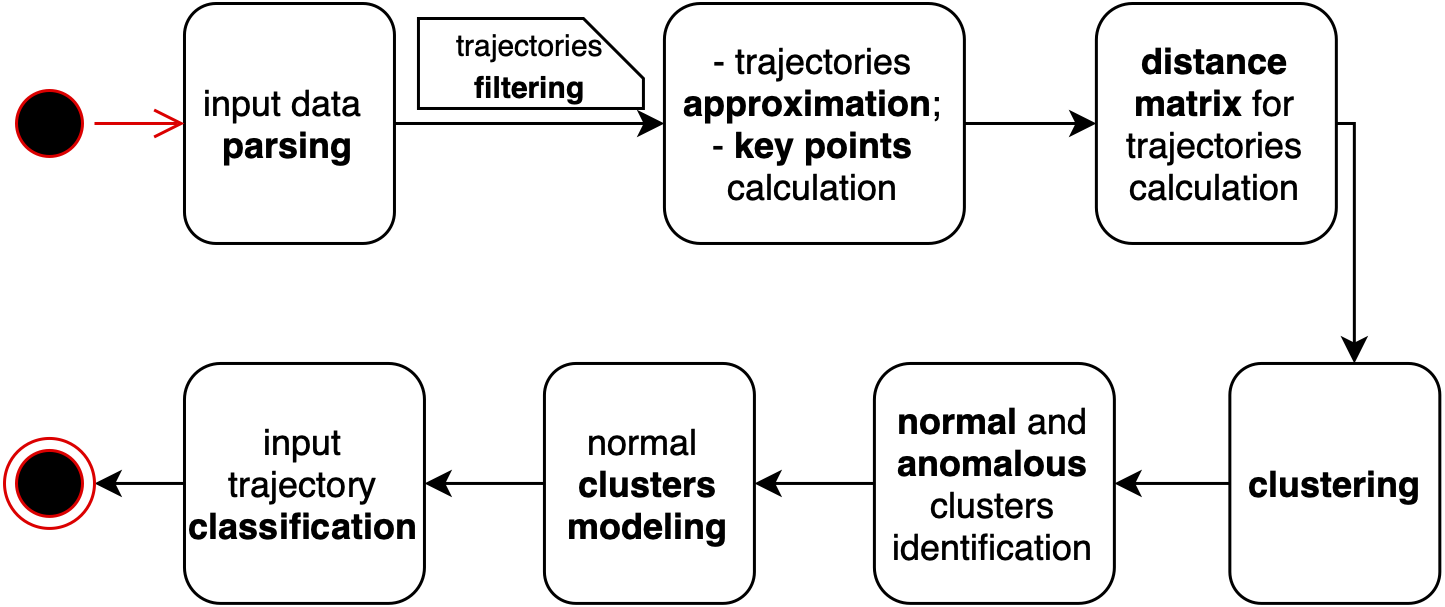
\includegraphics[width=0.8\textwidth]{images/flowchart.png}
	\caption{Basic workflow of the framework}
	\label{fig:flowchart}
\end{figure}

\section{Framework Architecture}

The architecture of the framework is based on an already discussed related work \cite{inproceedings:7_related_work} and consists of two phases (\ref{fig:str}):

\begin{itemize}
	\item \textit{offline} to perform clustering and extract frequent trajectories, and
	\item \textit{online} to classify the new trajectory as a normal or abnormal one.
\end{itemize}

\begin{figure}[!htb]
	\centering{}
	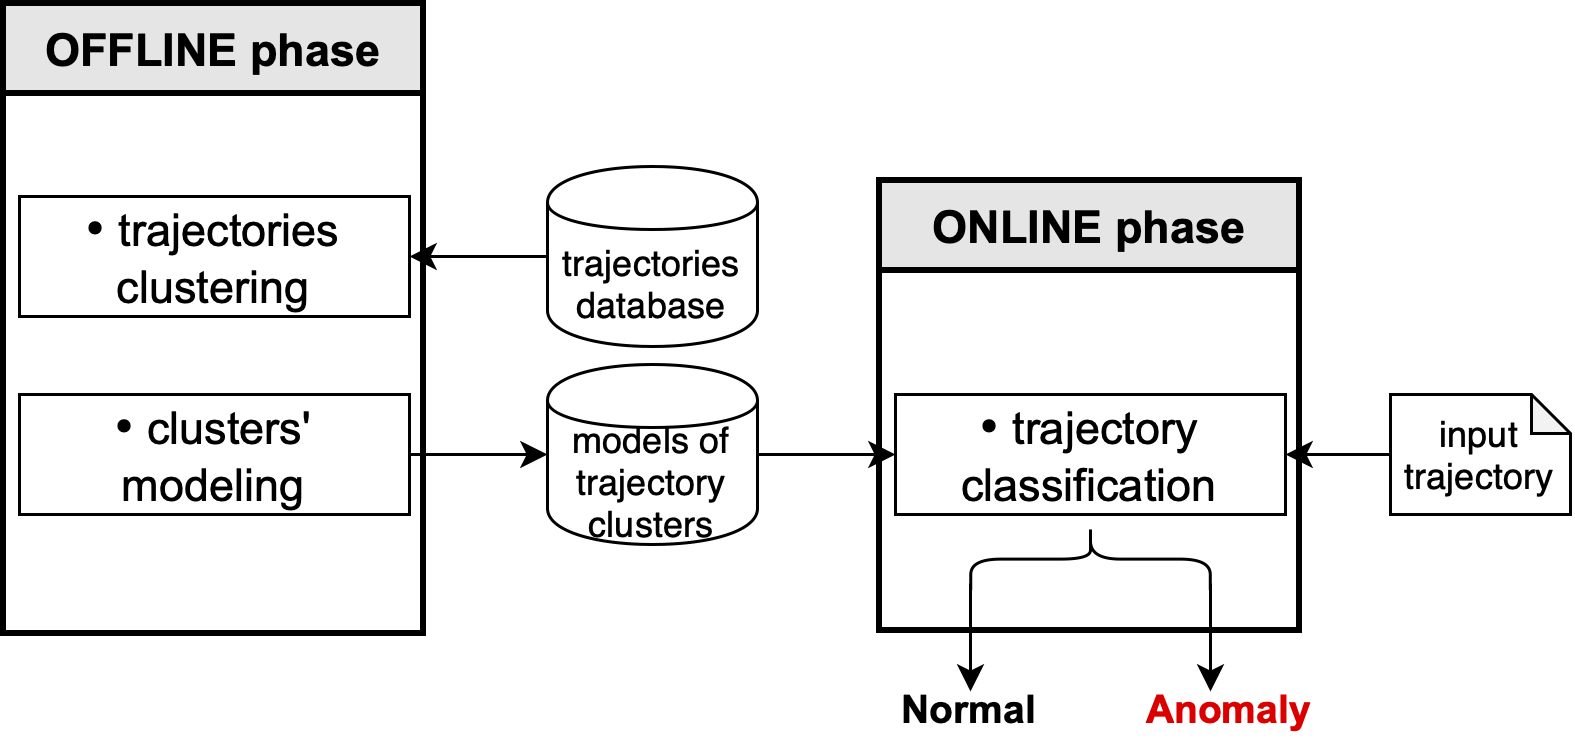
\includegraphics[width=0.8\textwidth]{images/str.png}
	\caption{Two-phased proposed approach}
	\label{fig:str}
\end{figure}

The implemented framework consists of several modules which are responsible for performing particular steps of the aforementioned workflow (Figure \ref{fig:proj-arch}):
\begin{itemize}
	\item \textit{entity} -- contains entity-classes for $Trajectory$, $TrajectoryPoint$, $Cluster$ and etc. objects;
	\item \textit{parsing} -- reading a 'txt'-file with input trajectories and parsing them to create $TrajectoryPoint$ and $Trajectory$ objects;
	\item \textit{csv} -- contains logic for reading and writing from/into 'csv'-files, is used to save calculated LCSS measures and load to proceed with clustering;
	\item \textit{approximation} -- performs an approximation of trajectories using a Polynomial regression;
	\item \textit{visualization} -- is responsible for visualization and saving the results, contains methods to read, edit, save $BufferedImage$'s;
	\item \textit{clustering} -- consists of a $Clustering$ class which contains methods to compute LCSS metric values, perform clustering of $Trajectory$ objects and create $Cluster$ objects;
	\item \textit{exception} -- contains exceptional classes hypothetically thrown in the framework (e.g. $TrajectoryParserException$);
	\item \textit{misc} -- contains utility classes needed to store constant values and basic methods.
\end{itemize}

\begin{figure}[!htb]
	\centering{}
	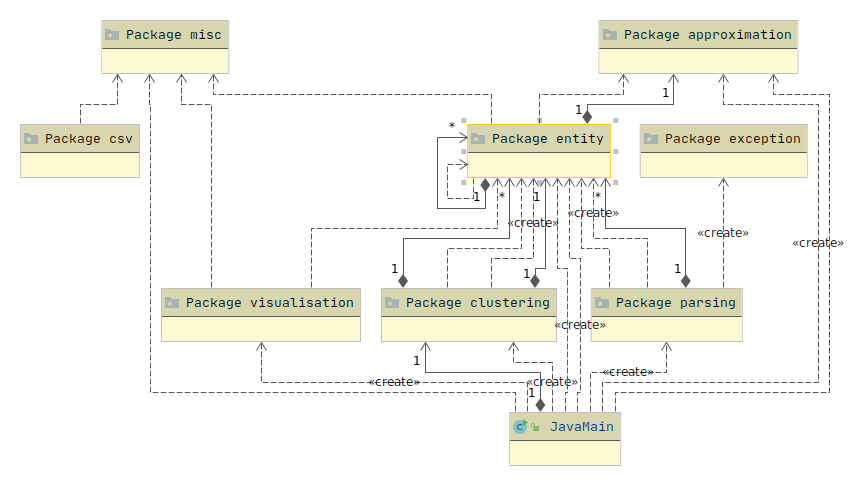
\includegraphics[width=0.8\textwidth]{images/proj-arch.png}
	\caption{Architecture of an implemented framework}
	\label{fig:proj-arch}
\end{figure}

\section{Agglomerative Hierarchical Clustering}

Clustering is done using an unsupervised agglomerative hierarchical clustering approach. The description of this approach is given in Algorithm \ref{algo:ahc-descr} \cite{inproceedings:7_related_work}.

\begin{algorithm}[!htb]
	\caption{Description of Agglomerative Hierarchical Clustering}
	\label{algo:ahc-descr}
	\SetAlgoLined
	\KwIn{A Database of Trajectories: trajectories}
	\KwOut{Clusters of Trajectories: clusters}
	\textit{Initialization:} \\
	- initialize the clusters with one trajectory in each cluster \\
	\textit{Clusters merging:}\\
	\While{number of clusters is greater than 1}{
		- calculate similarity matrix D between pairs of clusters based on single linkage approach using LCSS similarity measure;\\
		- find the smallest distance between clusters in D;\\
		- merge two clusters with the corresponding smallest distance into a single cluster;\\
		- remove two merged clusters;\\
	}
	
\end{algorithm}

As it was already mentioned, agglomerative hierarchical clustering methods suppose clusters joining, which requires the inter-cluster distance measure to be defined. In \cite{inproceedings:7_related_work} authors have performed evaluation of different linkage methods, including single link, complete link and average link. According to the performed tests, the single link method showed the best results and, in view of this, will be used as a linkage method in the current work.

Single link linkage method considers a minimum distance between two trajectories as an inter-cluster distance and can be summed up as \cite{inproceedings:7_related_work}:

\begin{equation} \label{eq:single_link}
D_{min}(C_i, C_j) = \min_{T_1 \in C_i, T_2 \in C_j} D_{LCSS}(T_1, T_2),
\end{equation} 

where ($C_i$, $C_j$) denote two clusters and ($T_1$, $T_2$) correspond to two trajectories from two clusters respectively.

\section{Clusters' modeling}

In order to perform a further classification of an input trajectory in a more efficient way, in the related work it was proposed to create cluster models (CM), or path models, for normal clusters. Model of a cluster can be described as a compact representation of it. Models of normal clusters can be considered as patterns of frequent trajectories since they represent the whole cluster of trajectories with the highest accuracy. 

Two main concepts of extracting a model from a cluster exist \cite{article:surv_cl_models}: 
\begin{itemize}
	\item taking a representative trajectory from the cluster. Such a trajectory is considered to be the center of a cluster. An easiest way to specify the representative trajectory is by defining only its centroid (cluster centroid, centroid path). As an extension a centroid can be augmented by a path envelope;
	\item estimating a model from the trajectories associated with the cluster by the use of probabilistic models, such as the Gaussian observation emission HMMs. Such method requires the trajectories to be preprocessed and is better to apply on probabilistically modeled trajectories.
\end{itemize}

In comparison with the second case, taking a representative trajectory for each cluster as a model is more simple, moreover, it does not require the trajectories to have the same number of trajectory points \cite{inproceedings:7_related_work}.

Authors in \cite{inproceedings:7_related_work} propose an easy to calculate way of modeling a cluster without any preprocessing of trajectories: a CM is a trajectory least of all distant from others and in view of this can be considered as a cluster center and representation. That means choosing a trajectory with a minimum average LCSS distance to other trajectories in this cluster (Formula \ref{eq:cm_traj}):

\begin{equation} \label{eq:cm_traj}
	CM(C) = \min\limits_{T \in C} \frac{1}{|C|} \sum_{T' \in C} D_{LCSS}(T, T')
\end{equation}


\section{Trajectories similarity}

It was mentioned before, that LCSS distance is used as a distance measure between trajectories to perform clustering. LCSS distance implies computing the Longest Common SubSequence between two input trajectories using two parameter values: $\delta$ and $\varepsilon$. 

Traditionally $\delta$ and $\varepsilon$ parameters are constant and defined in advance. However, in the developed framework in order to handle uncertainty of trajectory data coming from different position in respect to camera adaptive values of parameters are implemented. Parameters are functionally dependent on position of a moving object on a scene in respect to the camera. 

While considering the visualization of trajectories on sample images taken from the cameras, following can be deduced: since the bottom part of the image represent the region located closer to surveillance camera, moving objects on the upper part of the image are more distant from the camera and as a result are more densely located in respect to representation of each other on the image. $\varepsilon$ is responsible for the threshold controlling spatial remoteness of trajectory points while computing similarity distance. Consequently, it must be adapted to the remoteness and decrease as a trajectory point gets farther from the camera.

\todo{$\delta$ behaviour?}

LCSS calculation is described in Algorithm \ref{algo:lcss-descr}.
\todo{include $\delta$ and $\varepsilon$ as an input or calculate inside?}

\begin{algorithm}[!htb]
	\caption{Description of LCSS distance calculation}
	\label{algo:lcss-descr}
	\SetAlgoLined
	\KwIn{First trajectory: $T_1$,\newline
			Second trajectory: $T_2$,\newline
			Temporal remoteness threshold: $\delta$,\newline
			Spatial remoteness threshold: $\varepsilon$
	}
	\KwOut{LCSS distance for two trajectories}
	\Begin{
		// Initialization \\
		- calculate length of $T_1$\;
		- calculate length of $T_2$\;
		// LCSS similarity calculation \newline	
		\eIf {$T_1$ or $T_2$ is empty}{
			return 0;	
		}{\eIf {difference between X-coordinates < $\varepsilon$ \newline
			AND difference between Y-coordinates < $\varepsilon$ \newline
			AND difference between trajectory lengths < $\delta$}{
				- increase LCSS by 1\;
				- call recursive for trajectories excluding last points\;
			}{
				- calculate LCSS for first trajectory and second trajectory 	excluding last point\;
				- calculate LCSS for first trajectory excluding last point and second trajectory\;
				- take maximum between these LCSS values\;
			}
		}
		// LCSS distance calculation \\
		LCSS distance = 1 - LCSS similarity / minimum(input lengths)
	}
\end{algorithm}

\subsection{LCSS parameters adaptability}

The traditional LCSS measure supposed using a constant $\delta$ and $\varepsilon$ parameters and does not imply making them adaptive. However, one of the objectives in this work is investigating an opportunity to increase results accuracy by exploring a functional dependency between these parameters and a distance from the camera. Since camera is placed at a fixed location on an intersection, the problems caused by a perspective can take place. It can be seen from the Figure \ref{fig:tr_p} depicting the allocation of input trajectories that with distance from the camera, which is placed at the lower fore part of the image, trajectories become more densely located relative to each other (the input data will be described and depicted in the following chapter). In the case of a constant $\varepsilon$ value, which controls the threshold while testing the spatial equality of trajectory points, trajectory points of trajectories located far from camera (meaning they appear at the upper part of the sample images and are more densely located to each other) will be incorrectly considered as similar. This can contort the following analysis and skew the further clustering results.

The approach to make the parameters adaptive considered in this work is described in Algorithm \ref{algo:lcss-params-adapt}.

\begin{algorithm}[!htb]
	\caption{Adaptive LCSS parameters calculation}
	\label{algo:lcss-params-adapt}
	\SetAlgoLined
	\KwIn{First trajectory point: $TP_1$,\newline
		Second trajectory point: $TP_2$
	}
	\KwOut{Adaptive $\varepsilon$ value for $TP_1$ and $TP_2$}
	\Begin{
		// Initialization \\
		- compute location of a camera point ($CP$)\;
		- compute Euclidean distance for two pairs $d_1$($TP_1$, $CP$) and $d_2$($TP_2$, $CP$)\;
		- compute corresponding $\varepsilon_1$ and $\varepsilon_2$ values\;
		- take the min($\varepsilon_1$, $\varepsilon_2$) as a final $\varepsilon$ to compare $TP_1$ and $TP_2$.
	}
\end{algorithm}

In order to optimize the calculation of a distance to camera point and avoid recalculation of it multiple times during the LCSS computation algorithm, this distance is being calculated in advance and stored for each trajectory point.

\section{Measuring the Clusters Validity}

Since the goal of the current work is finding an optimal adaptive parameter values for similarity measure computation, it is necessary to analyze and compare the results after performing clustering. 

According to \cite{online:dunn_cl_valid} cluster validity measures can be classified as follows:
\begin{itemize}
	\item \textbf{Internal cluster validation} -- the result of performed clustering is being evaluated based on the input data clustered. It is based on an internal information and does not include references to external information.
	\item \textbf{External cluster validation} -- evaluation of clustering results is performed in accordance with externally known results, e.g. given class labels. Such validation is not appropriate for unsupervised clustering then no input labels are provided.
	\item \textbf{Relative cluster validation} -- evaluation of the clustering results is done by running the same algorithm using different input parameters, such as number of clusters, etc..
\end{itemize}

At the same time clustering is primarily an unsupervised data mining technique and the input data does not contain data labels. That leads to the necessity to test the resulting clusters in an unsupervised manner. 

One of the most widely used and known measures for evaluating clustering algorithms is a Dunn's Validity Index (DI), which was introduced by J. C. Dunn in 1974 in \cite{article:dunn_orig}. It is an internal evaluation metric which is intended to identify compact clusters with a small variance between cluster members which are well-separated between each other, meaning clusters are sufficiently distant from surrounding clusters in comparison with inter-cluster variance \cite{online:hier_clust_r}. Dunn's index is calculated as the ratio between the minimum inter-cluster distance $d_{min}$ to the maximum intra-cluster diameter $d_{max}$ and for $k$ number of clusters can be defined as follows (Formula \ref{eq:dunn-index}) \cite{article:quant_eval_perf_clust}:

\begin{equation} \label{eq:dunn-index}
	DI = \frac {d_{min}} {d_{max}} = \frac{\min\limits_{\substack{1 \leq i \leq k \\ i+1 \leq j \leq k}} dist(c_i, c_j)} {\max\limits_{1 \leq l \leq k} diam(c_l)}
\end{equation}

where minimum inter-cluster distance $d_{min}$ in accordance with the single linkage method refers to the minimal distance between two trajectories from different clusters. Maximum intra-cluster diameter $d_{max}$, or the largest within-cluster distance in other words, supposes computing the diameter of a cluster as a distance between its two farthermost trajectories \cite{inproceedings:clust_ind}. 

The sample description of a DI index for 3 clusters is given in Figure \ref{fig:di_sample}. According to this sample, Formula \ref{eq:dunn-index-sample} can be written out as follows:

\begin{equation} \label{eq:dunn-index-sample}
DI = \frac {d_{min}} {d_{max}} = \frac
	{\min ({dist_{min}}^1, {dist_{min}}^2, {dist_{min}}^3)}
	{\max ({diam_{max}}^1, {diam_{max}}^2, {diam_{max}}^3)}
\end{equation}

\begin{figure}[!htb]
	\centering{}
	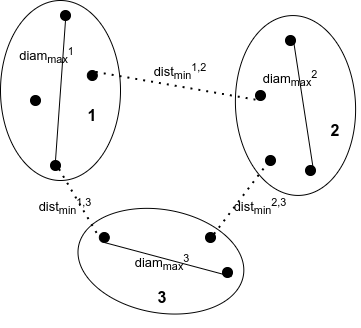
\includegraphics[width=0.5\textwidth]{images/di-sample.png}
	\caption{Explanation of DI}
	\label{fig:di_sample}
\end{figure}

Higher values of the DI indicates the better results of clustering. Trajectories, located far from each other inside one cluster, must be distinguishable from trajectories relating to other clusters. Values of DI close to 1 mean that minimum distances to trajectories from different clusters remain bigger than distance to farthermost trajectories from the same cluster. However, the computational cost of the DI is highly dependent on the data: the computation cost increases with the increase of number of clusters and dimensionality of the data \cite{online:dunn_cl_valid}.


\section{Trajectories Approximation}

However, notwithstanding that the LCSS similarity distance works with trajectories of arbitrary lengths and does not natively require the preprocessing of trajectories, the calculation of LCSS measure becomes extremely computationally expensive and time consuming with the growth of the trajectory length because of the recursiveness. For that reason it was decided to decrease the size of trajectories in the current work by approximation of trajectory data. That leads to the lose of accuracy but allows to get acceptable results in adequate amount of time.

The curve fitting concept is one of the standard approaches to perform approximation \cite{article:behav_form_extr}. The main task is finding an appropriate relation or law possibly existing between the input (independent) and output (dependent) variables from a given input data set of observed values. And the curve fitting is the process of expressing a relationship between variables in terms of algebraic equations. The main goal of the curve fitting is to find parameters for a model (equation or function) to fit to the experimental data. 

\subsection{Regression Analysis}

One of the widely used approaches appearing from curve fitting is a Regression Analysis, which is also considered as a form of predictive modeling approach and, according to the traditional definition, studies the relationship between a dependent variable (response) $Y$ and one or more independent variables $X$'s and tends to find trends in data. In other words it supposes ``using the relationship between variables to fit the best fit line or regression equation that can be used to make predictions'' \cite{online:intro_lr_pr}.

In order to simplify the relationship fitting procedure, it is usually assumed that the independent $X$ variables are measured without an error while the dependent $Y$ variables values are measured with some random error. For the data with a small ratio of the measurement error in an independent variable to the range of values of that variable, it is possible to use the least squares regression analysis with legitimacy \cite{article:behav_form_extr}.

A regression can be linear or polynomial (nonlinear, curvilinear) depending on the function the data is approximated with: linear regression refers to a relationship approximated by a straight line whereas curvilinear regression refers to a relationship following a curve. Due to a broader range of functions the polynomial regression can work with, it provides better approximation of the input relationship in comparison to linear regression \cite{online:intro_lr_pr}. Even if it is impossible to guess the type of function to use for approximation in advance, plotting the data and analyzing it to find some behavioral pattern, such as linear, quadratic or higher-order dependency, can be useful \cite{article:behav_form_extr}. 

\subsection{Polynomial Regression}

The visualization of input trajectory data is given in Figure \ref{fig:tr_p}. As it can be seen from the picture, neither the linear or $2\up{nd}$ order functions can not fit the data properly due to complexity of trajectory forms. For that reason it was decided to focus on approximation using higher-order polynomial regression. The evaluation of polynomial regression with different degrees will be given further and the following discussion and implementation will be intended to find a suitable $n\up{th}$ order polynomial equation and parameter values to represent each input trajectory as a `trajectory function'. Since trajectory data is represented by two-dimensional spatial data along with temporal data and it is necessary to approximate spatial information, $x$- and $y$-coordinates will be considered as dependent variables and $time$ will be used as an independent variable. Consequently, polynomial regression will be performed twice with two output polynomial functions representing $x(t)$ and $y(t)$ for each of the input trajectories $T$:

\begin{equation}\label{eq:regr-func}
	\forall\ T = [\ldots (x_i, y_i, t_i) \ldots] = > T(t) = 
		\begin{cases}
			x = x(t) \\
			y = y(t) \\
		\end{cases}
\end{equation}

Trajectories will be converted from a shape of a list of trajectory points into equations (time functions) defined in a geometrical space, which can represent approximately all of them. Taking key points of the representative polynomial can decrease the size of the trajectory therethrough reducing the total operational cost and computational complexity of LCSS calculation. Moreover, mathematical equations are able to store information in a dense form and apart from other advantages such a data reduction leads to consuming less amount of space and increasing the storage efficiency \cite{article:behav_form_extr}. Also so called built `trajectory functions's can provide interpolation and discover the missing data points.

